% !TEX encoding = UTF-8
% !TEX TS-program = pdflatex
% !TEX root = ../tesi.tex

%**************************************************************
\chapter{Sviluppo del progetto}
\label{cap:sviluppo}
%**************************************************************
\section{Analisi dei requisiti}
In questa sezione descrivo gli attori di sistema e come ho svolto l'analisi dei requisiti.
Quest'ultima, a sua volta, è suddivisa in due sotto-attività che sono: lo studio dei casi d'uso e la redazione delle \emph{user stories}.
Per ognuna di esse dedico una sezione e riporto solo le parti più rilevanti.

\subsection{Attori}
La figura \ref{fig:attori} riporta il diagramma \emph{\acrshort{uml}} che descrive la gerarchia degli attori del sistema. Dopo un'attenta analisi ho individuato: cinque \
attori principali e uno secondario. Gli attori principali da me individuati sono: l'utente non autenticato, l'utente non autorizzato, l'utente \
di tipo fornitore, l'utente di tipo personale e l'utente di tipo \emph{admin}. L'unico utente secondario che ho individuato è Google, in quanto, all'interno del sistema, \
utilizziamo \emph{Google SSO} come servizio di autenticazione. 

\begin{figure}[!ht]
  \begin{center}
    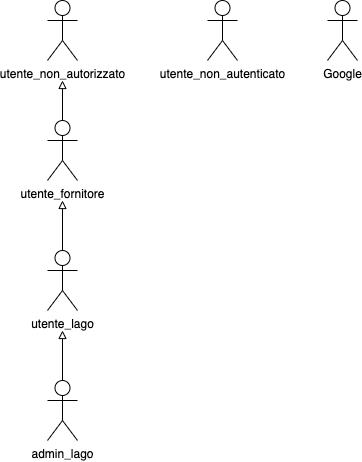
\includegraphics[scale=0.35]{usecase/attori}
    \caption{Gerarchia degli attori di sistema}
    \label{fig:attori}
  \end{center}
\end{figure}

\subsection{Casi d'uso}
Durante l'attività di analisi ho definito diversi diagrammi dei casi d'uso mediante il linguaggio \emph{\acrshort{uml}}.
Tutti i diagrammi sono contenuti all'interno del documento Analisi dei Requisiti aziendale. 
In questa sezione mostrerò solo il caso d'uso più generale, per dare un'idea di ciò che è possibile fare all'interno dell'applicazione. 
Ogni caso d'uso segue la seguente denominazione:

\begin{center}
  UC[codice]
\end{center}

dove per [codice] si intende un identificativo univoco del caso d'uso riportato in forma gerarchica. Per ogni caso d'uso, inoltre, vengono specificati:
\begin{itemize}
  \item Gli attori coinvolti;
  \item Una breve descrizione;
  \item La precondizione;
  \item La postcondizione;
  \item Lo scenario principale;
  \item Le eventuali estensioni.
\end{itemize}

\subsubsection{Caso d'uso UC0 - Scenario principale}
\begin{figure}[!ht]
  \begin{center}
    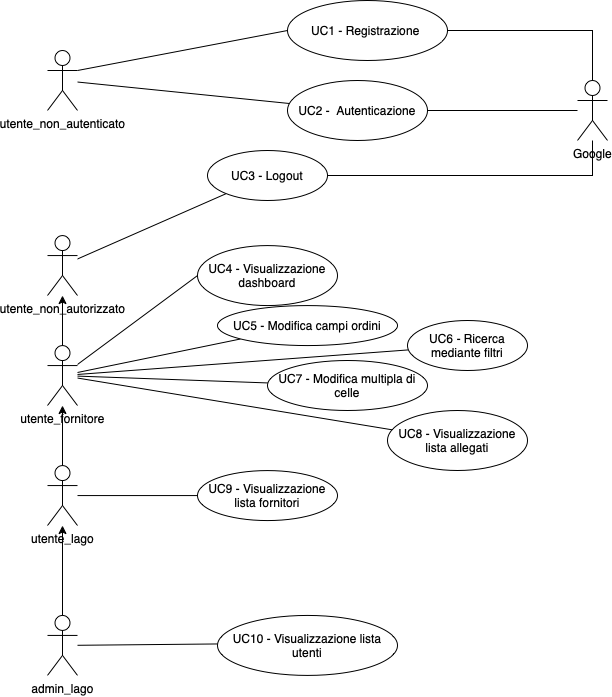
\includegraphics[scale=0.38]{usecase/main-scenario}
    \caption{UC0: Scenario principale}
    \label{fig:uc0}
  \end{center}
\end{figure}

\begin{itemize}
  \item \textbf{Attori:} utente non autenticato, utente autenticato, utente di tipo fornitore, utente di tipo personale e utente di tipo \emph{admin};
  \item \textbf{Descrizione:} nella schermata principale un utente non autenticato può autenticarsi, o registrarsi, tramite l'apposito pulsante che reindirizza l'utente al \emph{form} di Google. Un utente non autorizzato può effettuare il \emph{logout} dalla piattaforma. Un utente di tipo fornitore, oltre alle funzionalità dell'utente non autorizzato, ha la possibilità di:\
    \begin{itemize}
      \item visualizzare la \emph{dashboard};
      \item modificare una riga;
      \item effettuare la ricerca mediante filtri;
      \item effettuare la modifica multipla di celle;
      \item visualizzare gli allegati relativi ad un ordine.
    \end{itemize}
    Un utente di tipo personale, oltre alle funzionalità dell'utente fornitore, può visualizzare la lista dei fornitori. Un utente di tipo \emph{admin}, infine, oltre alle funzionalità dell'utente di tipo personale, può visualizzare la lista degli utenti registrati sulla piattaforma;
  \item \textbf{Precondizione:} il sistema è avviato e mostra la pagina principale dell'applicazione;
  \item \textbf{Postcondizione:} il sistema ha ricevuto tutte le informazioni dall'utente sulle operazioni che vuole eseguire;
  \item \textbf{Scenario principale:} 
    \begin{itemize}
      \item L'utente non autenticato può effettuare la registrazione alla piattaforma (UC1);
      \item L'utente non autenticato può effettuare l'autenticazione (UC2);
      \item L'utente non autorizzato, l'utente di tipo fornitore, l'utente di tipo personale e l'utente di tipo \emph{admin} possono effettuare il \emph{logout} (UC3);
      \item L'utente di tipo fornitore, l'utente di tipo personale e l'utente di tipo \emph{admin} possono visualizzare la \emph{dashboard} (UC4);
      \item L'utente di tipo fornitore, l'utente di tipo personale e l'utente di tipo \emph{admin} possono modificare un campo di un ordine (UC5);
      \item L'utente di tipo fornitore, l'utente di tipo personale e l'utente di tipo \emph{admin} possono effettuare la ricerca mediante filtri (UC6);
      \item L'utente di tipo fornitore, l'utente di tipo personale e l'utente di tipo \emph{admin} possono effettuare la modifica multipla di ordini (UC7);
      \item L'utente di tipo fornitore, l'utente di tipo personale e l'utente di tipo \emph{admin} possono visualizzare gli allegati di un ordine (UC8);
      \item L'utente di tipo personale e l'utente di tipo \emph{admin} possono visualizzare la lista dei fornitori (UC9);
      \item L'utente di tipo \emph{admin} può visualizzare la lista degli utenti registrati nella piattaforma (UC10).
    \end{itemize}
\end{itemize}

\subsection{\emph{User Stories}}
Grazie alla definizione dei casi d'uso ho estratto le \emph{user stories}, e ho provveduto allo svolgimento delle attività in esse specificate. 
In totale ne ho individuate 16: 12 obbligatorie e 4 desiderabili.
Di seguito sono riportate quelle relative alle funzionalità principali.

\subsubsection{Login con \emph{Google SSO} (5)}
Come utente non autenticato, voglio poter accedere alla piattaforma mediante \emph{Google SSO}. \\
\emph{Tasks:}
\begin{itemize}
  \item \emph{\Gls{backend}}:
    \begin{itemize}
      \item Creazione \emph{collection users};
      \item Implementazione chiamata \emph{\acrshort{api}} di \emph{Google SSO};
      \item Se l'utente non è presente, memorizzare il \emph{token} e metterlo in stato \emph{"disabled"};
      \item Verifica della validità del \emph{token}.
    \end{itemize}
  \item \emph{\Gls{frontend}}:
    \begin{itemize}
      \item Implementazione della chiamata all'\emph{\acrshort{api}} di \emph{login} del \emph{\gls{backend}};
      \item Creazione della sessione utente;
      \item Reindirizzamento alla \emph{dashboard}.
    \end{itemize}
\end{itemize}

\subsubsection{Visualizzazione lista fornitori (5)}
Come utente di tipo personale, voglio visualizzare la lista di tutti i fornitori abilitati. \\
\emph{Tasks:}
\begin{itemize}
  \item \emph{\Gls{backend}}:
    \begin{itemize}
      \item Creazione \emph{collection suppliers};
      \item Verifica dei permessi di esecuzione dell'\emph{\acrshort{api}};
      \item Implementazione dell'\emph{\acrshort{api} "get suppliers"}.
    \end{itemize}
  \item \emph{\Gls{frontend}}:
    \begin{itemize}
      \item Implementazione della chiamata all'\emph{\acrshort{api} "get suppliers"} del \emph{\gls{backend}};
      \item Visualizzazione della lista dei fornitori.
    \end{itemize}
\end{itemize}

\subsubsection{Visualizzazione fornitore (5)}
Come utente di tipo personale o utente di tipo fornitore, voglio visualizzare la griglia di un fornitore. \\
\emph{Tasks:}
\begin{itemize}
  \item \emph{\Gls{backend}}:
    \begin{itemize}
      \item Definizione della struttura della configurazione di una colonna;
      \item Definizione della struttura della configurazione per il contenuto della colonna;
      \item Creazione \emph{collection order-rows};
      \item Verifica dei permessi di esecuzione dell'\emph{\acrshort{api}};
      \item Implementazione dell'\emph{\acrshort{api} "get order-rows"} di un fornitore.
    \end{itemize}
  \item \emph{\Gls{frontend}}:
    \begin{itemize}
      \item Implementazione della chiamata all'\emph{\acrshort{api} "get order-rows"} del \emph{\gls{backend}};
      \item Visualizzazione della griglia con i dati degli ordini di un fornitore.
    \end{itemize}
\end{itemize}

\subsubsection{Modifica dei campi di un ordine (5)}
Come utente di tipo personale o utente di tipo fornitore, voglio poter modificare un campo di un ordine. \\
\emph{Tasks:}
\begin{itemize}
  \item \emph{\Gls{backend}}:
    \begin{itemize}
      \item Verifica dei permessi di esecuzione dell'\emph{\acrshort{api}};
      \item Implementazione dell'\emph{\acrshort{api} "update order-row"} per un ordine di un fornitore.
    \end{itemize}
  \item \emph{\Gls{frontend}}:
    \begin{itemize}
      \item Validazione del campo modificato;
      \item Visualizzazione di un errore in caso di valore non valido;
      \item Implementazione della chiamata all'\emph{\acrshort{api} "update order-row"} del \emph{\gls{backend}};
      \item Visualizzazione della griglia con i dati degli ordini aggiornati.
    \end{itemize}
\end{itemize}

\subsubsection{Visualizzazione della lista degli utenti (5)}
Come utente \emph{admin}, voglio poter visualizzare la lista degli utenti registrati. \\
\emph{Tasks:}
\begin{itemize}
  \item \emph{\Gls{backend}}:
    \begin{itemize}
      \item Verifica dei permessi di esecuzione dell'\emph{\acrshort{api}};
      \item Implementazione dell'\emph{\acrshort{api} "get users"}.
    \end{itemize}
  \item \emph{\Gls{frontend}}:
    \begin{itemize}
      \item Implementazione della chiamata all'\emph{\acrshort{api} "get users"} del \emph{\gls{backend}};
      \item Visualizzazione della lista degli utenti.
    \end{itemize}
\end{itemize}

\subsubsection{Visualizzazione della lista degli allegati (5)}
Come utente di tipo personale o utente di tipo fornitore, voglio poter visualizzare la lista degli allegati relativi ad un ordine. \\
\emph{Tasks:}
\begin{itemize}
  \item \emph{\Gls{backend}}:
    \begin{itemize}
      \item Verifica dei permessi di esecuzione dell'\emph{\acrshort{api}};
      \item Implementazione del sistema per l'invio dei file allegati da visualizzare;
      \item Implementazione dell'\emph{\acrshort{api} "get attachments"} di un ordine.
    \end{itemize}
  \item \emph{\Gls{frontend}}:
    \begin{itemize}
      \item Implementazione della chiamata all'\emph{\acrshort{api} "get attachments"} del \emph{\gls{backend}};
      \item Visualizzazione della lista degli allegati di un ordine.
    \end{itemize}
\end{itemize}

%**************************************************************
\section{Progettazione architetturale}

L'applicazione è costituita da due parti principali: il \emph{\gls{frontend}} e il \emph{\gls{backend}}, che costituiscono rispettivamente il \emph{client} e il \emph{server} nell'architettura \emph{client-server}. \
All'interno di questa architettura, il \emph{\gls{frontend}} ha il compito di interagire con l'utente e di mostrare i dati ottenuti dal \emph{server}. Il \emph{\gls{backend}}, invece, fornisce le \emph{\acrshort{api}} \
per poter svolgere determinate operazioni e ottenerne i risultati. Come si può vedere dalla figura \ref{fig:client-server}, che raffigura il flusso di comunicazione in questa architettura, entrambi i componenti sono indipendenti tra loro e comunicano utilizzando richieste \emph{\acrshort{http}}. Possono essere di diversi tipi a \
seconda dell'operazione che intendiamo svolgere: 
\begin{itemize}
  \item \textbf{\emph{GET}:} per ottenere i dati dal \emph{server};
  \item \textbf{\emph{POST}:} per caricare dei dati sul \emph{server};
  \item \textbf{\emph{PUT}:} per aggiornare i dati sul \emph{server};
  \item \textbf{\emph{DELETE}:} per eliminare dei dati sul \emph{server}.
\end{itemize} 

\begin{figure}[!ht]
  \begin{center}
    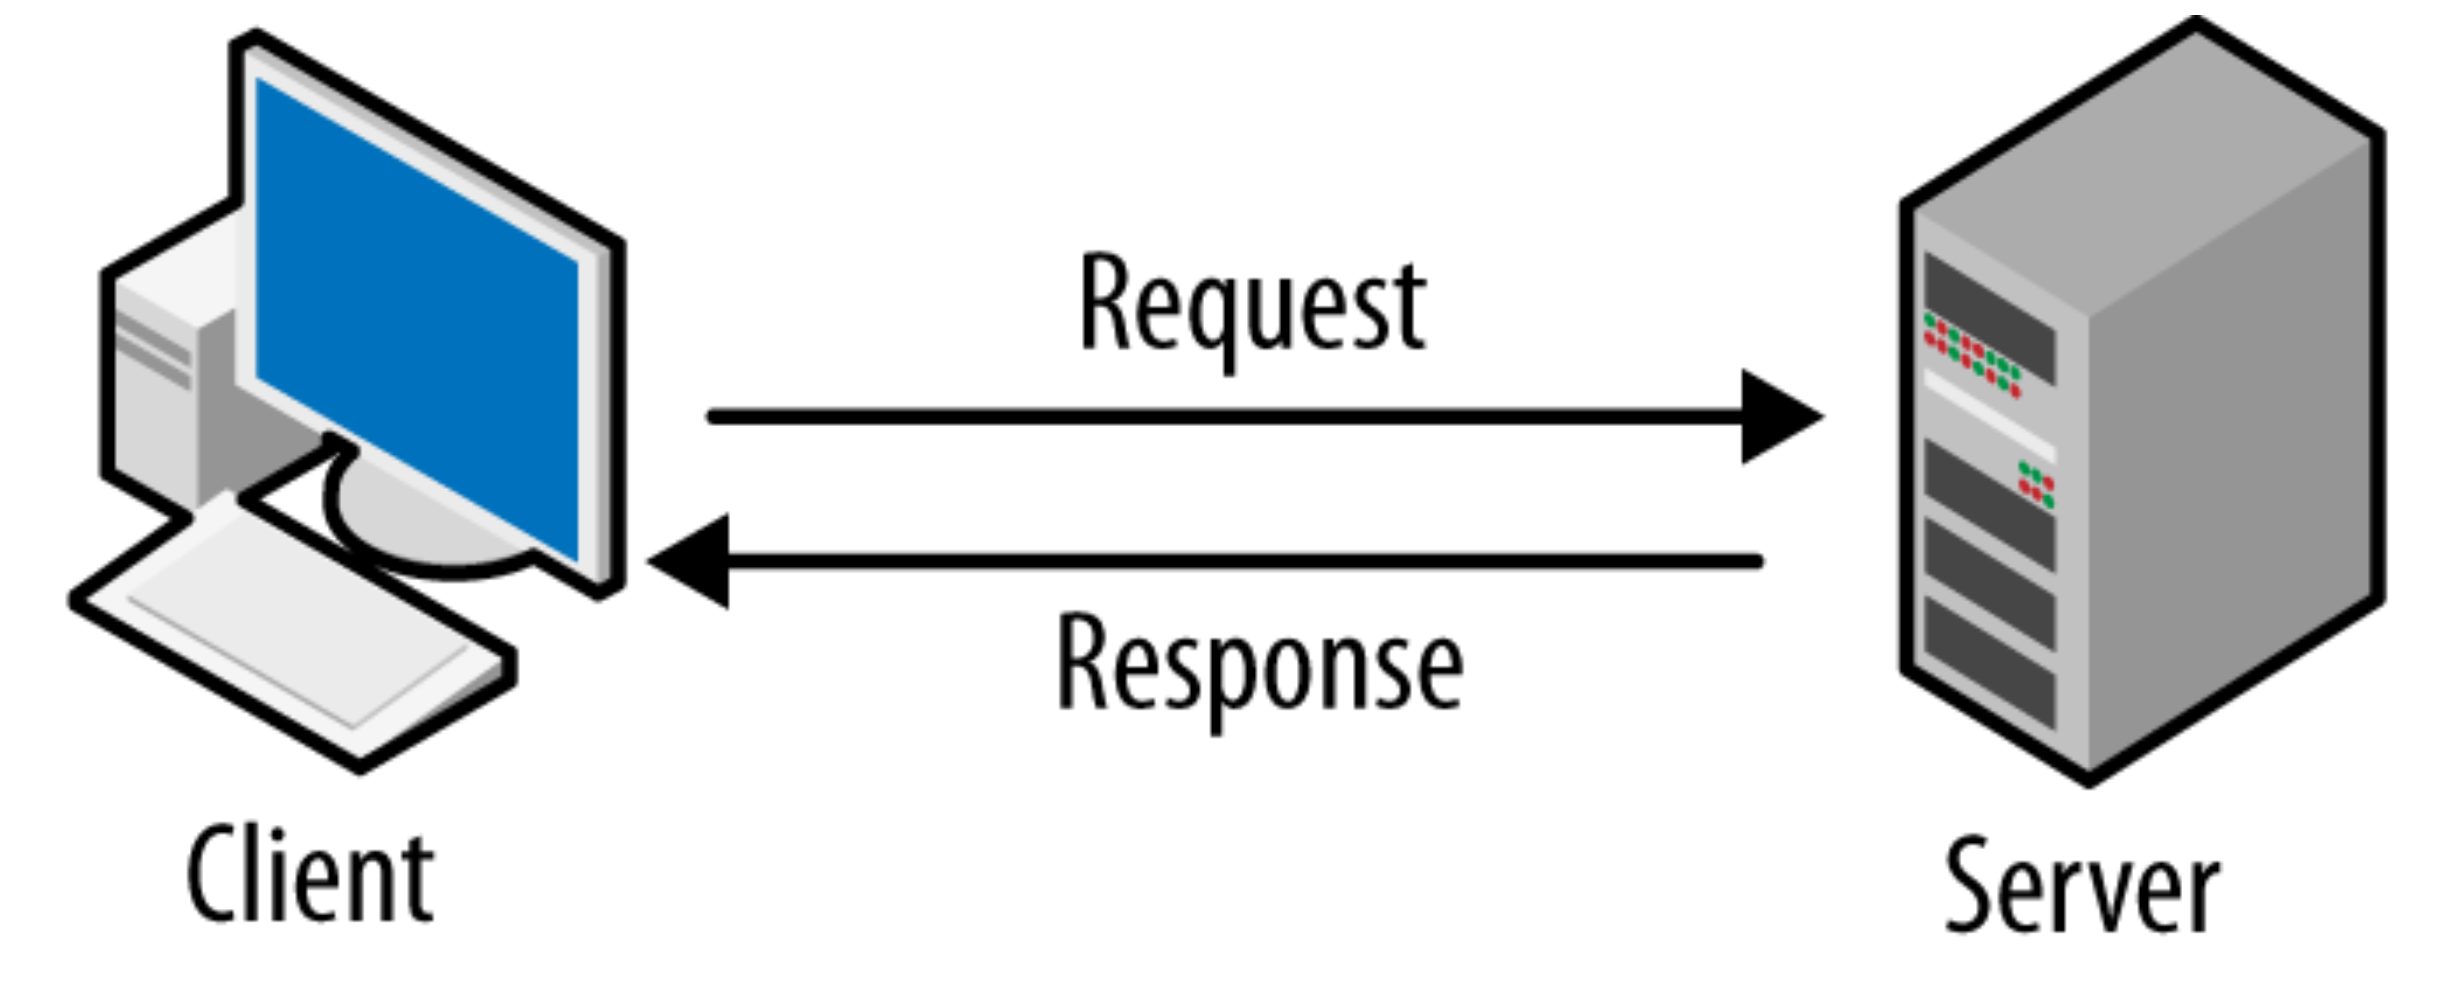
\includegraphics[scale=0.1]{design/client-server}
    \caption{Flusso di comunicazione \emph{client-server}}
    \label{fig:client-server}
  \end{center}
\end{figure}

Come si evince dalla figura \ref{fig:general-design}, che mostra lo schema architetturale generale, l'applicazione è costituita da tre \emph{packages} principali:
\begin{itemize}
  \item \textbf{\emph{edi-api}:} contiene i \emph{packages} necessari, per il funzionamento del \emph{\gls{backend}};
  \item \textbf{\emph{edi-ui}:} contiene i \emph{packages} necessari, per il funzionamento del \emph{\gls{frontend}};
  \item \textbf{\emph{edi-commons}:} contiene i \emph{packages}, che vengono riutilizzati sia nel \emph{\gls{backend}} che nel \emph{\gls{frontend}}.
\end{itemize}

\begin{figure}[!ht]
  \begin{center}
    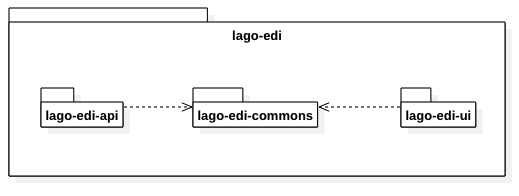
\includegraphics[scale=1, width=\textwidth]{design/general}
    \caption{Architettura generale dell'applicazione}
    \label{fig:general-design}
  \end{center}
\end{figure}
\newpage

L'applicazione, per funzionare, necessita dell'utilizzo di alcune librerie e \emph{frameworks} esterni. Questi garantiscono l'utilizzo di alcune funzionalità che \
permettono di velocizzare il lavoro e di svolgerlo in maniera più ordinata e sicura. Quelli che ho utilizzato all'interno del progetto, suddivisi per \emph{package}, sono:
\begin{itemize}
  \item \textbf{edi-api}
    \begin{itemize}
      \item \textbf{\emph{express}:} è il \emph{framework} su cui si basa l'intera applicazione \emph{\gls{backend}}, fornisce le basi per la creazione del \emph{server} e del \emph{routing};
      \item \textbf{\emph{mongoose}:} è una libreria per creare i modelli degli oggetti che vengono memorizzati su \emph{\textbf{MongoDB}}, inoltre, permette di eseguire le \emph{query} per manipolare i dati del \emph{database};
      \item \textbf{\emph{passport}:} è una libreria che rende disponibile dei \emph{middlewares} per facilitare l'implementazione dell'autenticazione su applicazioni basate su \emph{\textbf{express}};
      \item \textbf{\emph{inversify}:} è una libreria che permette di implementare applicazioni che sfruttano il \emph{design pattern Dependency Injection} con \emph{\acrfull{ioc}};
      \item \textbf{\emph{googleapis}:} è una libreria utilizzata per usufruire delle \emph{\acrshort{api}} di Google. Nello specifico, ho utilizzato questa libreria per implementare l'autenticazione degli utenti;
      \item \textbf{\emph{joi}:} è una libreria che permette di definire degli schemi per validare i dati in ingresso.
    \end{itemize}
  \item \textbf{edi-ui}
    \begin{itemize}
      \item \textbf{\emph{fuse.js}:} è una libreria che facilita l'implementazione delle funzionalità di ricerca lato \emph{\gls{frontend}};
      \item \textbf{\emph{styled-components}:} è una libreria che consente di definire dei componenti per la \emph{\gls{ui}} riutilizzabili e con stile personalizzato, senza l'utilizzo di file dedicati riducendo le dimensioni del progetto;
      \item \textbf{\emph{react-data-grid}:} è una libreria che fornisce i componenti per la creazione di griglie, uno dei componenti più importanti dell'applicazione \emph{\gls{frontend}};
      \item \textbf{\emph{react-query}:} è una libreria per applicazioni basate su \emph{\textbf{React}}, che fornisce le primitive di rete, per poter interagire con il \emph{\gls{backend}};
      \item \textbf{\emph{formik}:} è una libreria per applicazioni basate su \emph{\textbf{React}}, che facilita la creazione di \emph{form} per l'invio di dati inseriti dall'utente;
      \item \textbf{\emph{react}:} è la libreria su cui si basa l'intera applicazione \emph{\gls{frontend}}, permette la realizzazione di \emph{\acrfullpl{ui}} basate su componenti.
    \end{itemize}
\end{itemize} 

Per gestire le versioni di rilascio del prodotto, l'installazione e l'aggiornamento delle dipendenze esterne ho impiegato \emph{\textbf{lerna.js}}: un \emph{tool} che facilita la gestione di progetti composti da più \emph{packages}.

%**************************************************************
\section{Progettazione di dettaglio}

\subsection{Architettura del \emph{\gls{backend}}}
Addentrandoci nell'architettura del \emph{package} \textbf{edi-api}, come mostra la figura \ref{fig:be-design}, possiamo notare come esso sia costituito dai seguenti \emph{packages}:
\begin{itemize}
  \item \textbf{\emph{controllers}:} contiene tutti i componenti per fornire una risposta alle richieste \emph{\acrshort{http}} in ingresso. Costituisce la \emph{application logic};
  \item \textbf{\emph{middlewares}:} contiene tutte le funzioni da eseguire prima dell'esecuzione del \emph{controller};
  \item \textbf{\emph{services}:} contiene tutti i componenti necessari per fornire un servizio ai \emph{controllers};
  \item \textbf{\emph{repositories}:} contiene tutti i componenti che si occupano di interagire con il \emph{database};
  \item \textbf{\emph{models}:} contiene tutte le classi che costituiscono le tipologie di dati utilizzati nell'applicazione.
\end{itemize}

\begin{figure}[!ht]
  \begin{center}
    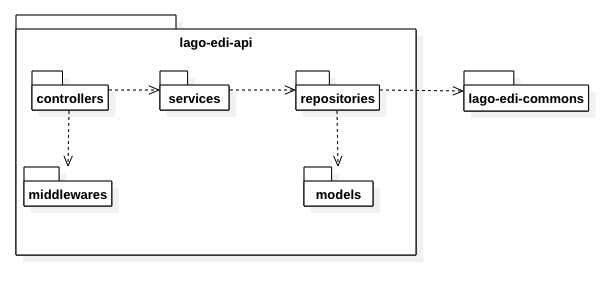
\includegraphics[scale=0.45]{design/backend}
    \caption{Architettura del \emph{\gls{backend}}}
    \label{fig:be-design}
  \end{center}
\end{figure}

L'intero \emph{package} è costituito da 22 classi e 13 interfacce.

\subsubsection{\emph{Design pattern} utilizzati}
Di seguito descrivo i \emph{design pattern} che ho utilizzato nell'architettura del \emph{\gls{backend}}. 
Per ognuno di essi descrivo lo scopo dell'utilizzo e il contesto di applicazione fornendo, inoltre, un diagramma che ne dimostri l'applicazione.
\begin{itemize}
  \item \textbf{\emph{\acrlong{mvc}}:} 
  la figura \ref{fig:mvc-pattern} fornisce una rappresentazione grafica del \emph{design pattern} architetturale \emph{\acrshort{mvc}}. Quest'ultimo, viene utilizzato per mantenere separati i compiti dei diversi componenti,
  che interpretano i tre ruoli principali: \emph{Model, View} e \emph{Controller}. Nel contesto applicativo, il \emph{pattern \acrshort{mvc}}, costituisce l'architettura generale del \emph{\gls{backend}}, questo perché il
  \emph{framework \textbf{express}} è basato su tale architettura. Durante l'implementazione non è stata implementata alcuna \emph{view}, in quanto, il \emph{\gls{backend}} si preoccupa esclusivamente di rendere disponibili 
  le \emph{\acrshort{api}} al \emph{\gls{frontend}} e quindi, risulta inutile, per questo motivo nella figura sottostante è evidenziata in rosso.

  \begin{figure}[!ht]
    \begin{center}
      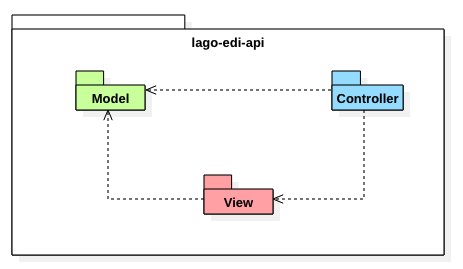
\includegraphics[scale=0.45]{design/patterns/mvc}
      \caption{Contesto di utilizzo del \emph{design pattern \acrshort{mvc}}}
      \label{fig:mvc-pattern}
    \end{center}
  \end{figure}
  \item \textbf{\emph{Dependency Injection}:}
  la figura \ref{fig:di-pattern} rappresenta il diagramma delle classi del \emph{design pattern} architetturale \emph{Dependency Injection}. Questo \emph{design pattern} è utilizzato per separare il comportamento di un componente dalla 
  risoluzione delle sue dipendenze, le quali, in questo modo, vengono minimizzate. Nel contesto applicativo, viene impiegato nell'architettura generale del
  \emph{package} \textbf{edi-api} per ottenere \emph{software} più facile da testare e manutenere. 

  \begin{figure}[!ht]
    \begin{center}
      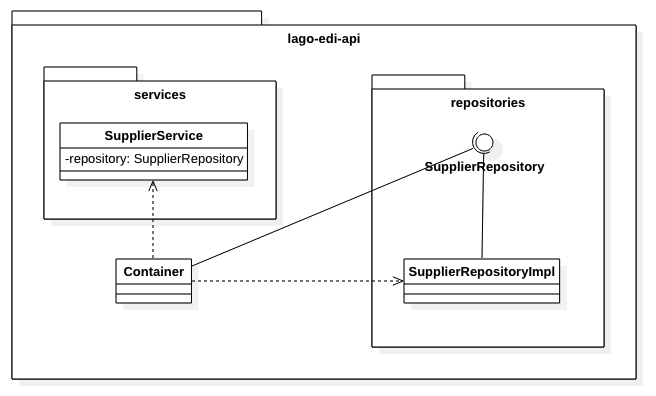
\includegraphics[scale=0.30]{design/patterns/di}
      \caption{Contesto di utilizzo del \emph{design pattern Dependency Injection}}
      \label{fig:di-pattern}
    \end{center}
  \end{figure}
\end{itemize}

\newpage
\subsection{Architettura del \emph{\gls{frontend}}}
La figura \ref{fig:fe-design} fornisce una rappresentazione grafica dell'architettura relativa al \emph{\gls{frontend}}. \
Il \emph{package} \textbf{edi-ui} è composto dai seguenti \emph{subpackages}:
\begin{itemize}
  \item \textbf{\emph{views}:} contiene tutte le pagine che il \emph{\gls{frontend}} deve mostrare all'utente;
  \item \textbf{\emph{contexts}:} contiene tutte le classi per gestire lo stato globale;
  \item \textbf{\emph{services}:} contiene tutti i componenti necessari per ottenere i dati dal \emph{\gls{backend}};
  \item \textbf{\emph{components}:} contiene tutti i componenti necessari per il \emph{rendering} delle pagine;
  \item \textbf{\emph{interfaces}:} contiene tutte le interfacce per la configurazione dei componenti della \emph{view}.
\end{itemize}

\begin{figure}[!ht]
  \begin{center}
    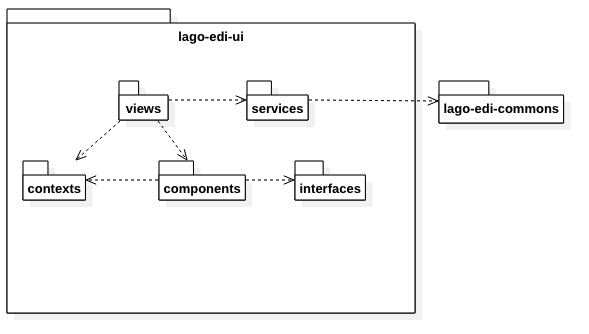
\includegraphics[scale=0.45]{design/frontend}
    \caption{Architettura del \emph{\gls{frontend}}}
    \label{fig:fe-design}
  \end{center}
\end{figure}

L'intero \emph{package} è costituito da 1 classe e 42 interfacce.

\subsubsection{\emph{Design pattern} utilizzati}
Di seguito descrivo i \emph{design pattern} che ho utilizzato nell'architettura del \emph{\gls{frontend}}. 
Per ognuno di essi descrivo lo scopo dell'utilizzo e il contesto di applicazione fornendo, inoltre, un diagramma che ne dimostri l'applicazione.
\begin{itemize}
  \item \textbf{\emph{Builder}:}
  la figura \ref{fig:builder-pattern} mostra il diagramma relativo al \emph{design pattern} creazionale \emph{Builder}. Questo \emph{design pattern}, permette di separare la costruzione di un oggetto complesso dalla
  sua rappresentazione e fornisce un controllo migliore del processo di costruzione, in quanto fornisce una costruzione \emph{step-by-step}. Nel contesto applicativo, è impiegato per la creazione delle colonne
  che compongono la griglia di un fornitore. Grazie al suo utilizzo, l'applicazione sarà in grado di creare nuove tipologie di colonne, senza apportare eccessive modifiche.

  \begin{figure}[!ht]
    \begin{center}
      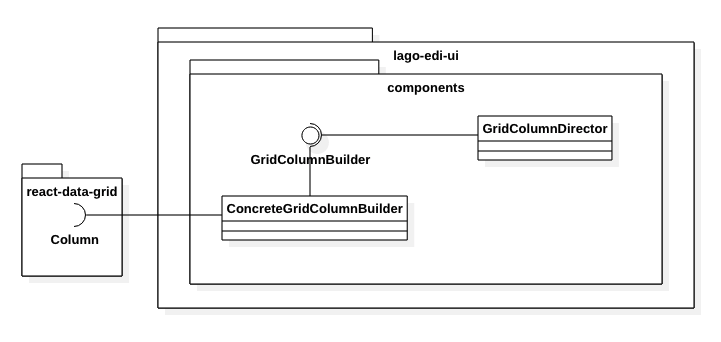
\includegraphics[scale=0.35]{design/patterns/builder}
      \caption{Contesto di utilizzo del \emph{design pattern Builder}}
      \label{fig:builder-pattern}
    \end{center}
  \end{figure}
  \newpage
  \item \textbf{\emph{Factory}:}
  la figura \ref{fig:factory-pattern} mostra il diagramma relativo al \emph{design pattern} creazionale \emph{Factory}. Quest'ultimo separa la creazione di un oggetto dalla sua rappresentazione, senza esporre la logica 
  di creazione. Nel contesto applicativo, viene adottato per la costruzione dei seguenti componenti della griglia del fornitore: 
  \begin{itemize}
    \item le celle;
    \item gli \emph{editor} delle celle;
    \item i \emph{formatter} delle celle.
  \end{itemize}

  \begin{figure}[!ht]
    \begin{center}
      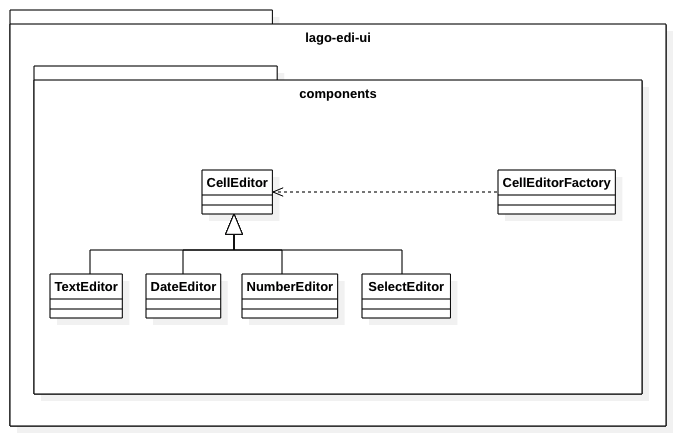
\includegraphics[scale=0.35]{design/patterns/factory}
      \caption{Contesto di utilizzo del \emph{design pattern Factory}}
      \label{fig:factory-pattern}
    \end{center}
  \end{figure}
\end{itemize}

\subsection{Struttura del \emph{database}}
Come \emph{database} ho utilizzato il \emph{\acrshort{dbms} NoSQL \textbf{MongoDB}}, mentre, per interagire con esso, ho impiegato la libreria \textbf{mongoose}. 
La figura \ref{fig:db-design} mostra il diagramma \emph{\acrshort{er}} del \emph{database} che ho realizzato utilizzando l'applicazione \textbf{\href{https://dbdiagram.io/}{dbdiagram.io}}. 
Di seguito fornisco una breve descrizione di ogni \emph{collection} del \emph{database}:

\begin{itemize}
  \item \textbf{\emph{users}:} memorizza tutti i dati degli utenti, compreso il fornitore a cui ha accesso, nel caso esso sia di tipo fornitore;
  \item \textbf{\emph{suppliers}:} memorizza i dati dei fornitori, inclusa la configurazione delle colonne della tabella;
  \item \textbf{\emph{order\_rows}:} memorizza i dati di tutti gli ordini relativi ad ogni fornitore.
\end{itemize}

\begin{figure}[!ht]
  \begin{center}
    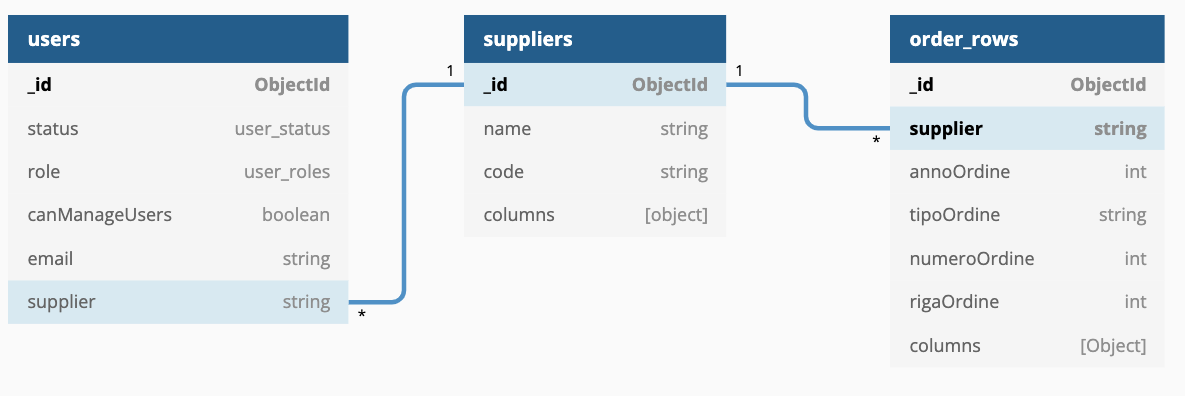
\includegraphics[scale=0.28]{design/database}
    \caption{Schema del \emph{database}}
    \label{fig:db-design}
  \end{center}
\end{figure}

\subsection{Diagrammi di sequenza}
Questa sezione riporta uno dei diagrammi di sequenza realizzati, durante il periodo di \emph{stage}, mediante l'utilizzo del \emph{software \textbf{StarUML}}.
La figura \ref{fig:auth-sequence} mostra il diagramma di sequenza relativo all'autenticazione, il più importante che ho realizzato, e che mi ha permesso di implementare la soluzione migliore possibile.

\begin{figure}[!ht]
  \begin{center}
    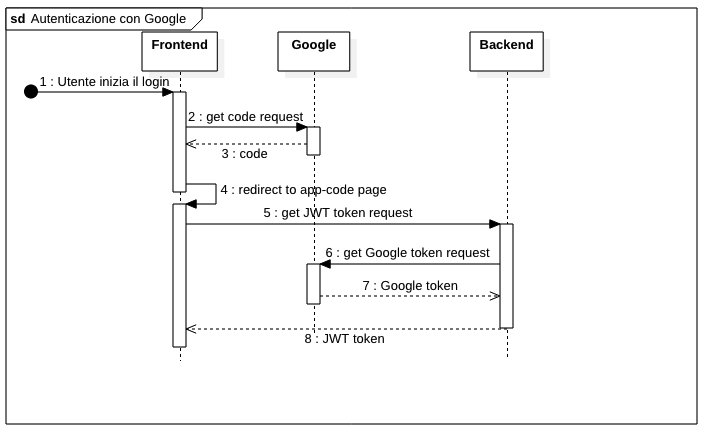
\includegraphics[scale=1, width=\textwidth]{design/auth-sequence}
    \caption{Diagramma di sequenza per l'autenticazione con Google}
    \label{fig:auth-sequence}
  \end{center}
\end{figure}

%**************************************************************
\section{Verifica e validazione}
In questa sezione descrivo le attività di verifica e validazione, svolte durante il periodo di \emph{stage}.
L'attività di verifica, a sua volta, è suddivisa in due sotto-attività che sono: l'analisi statica e l'analisi dinamica, per ognuna delle quali dedico una sezione.

\subsection{Analisi statica}
L'analisi statica permette di valutare la correttezza dei componenti, senza la loro esecuzione.
Durante il processo di sviluppo, ho utilizzato alcuni strumenti di analisi statica, per individuare gli errori più facilmente. Di seguito fornisco un elenco degli strumenti utilizzati:
\begin{itemize}
  \item \textbf{\textbf{WebStorm}:} questo \emph{\acrshort{ide}} permette di visualizzare \emph{warning} ed errori presenti all'interno del codice;
  \item \textbf{\textbf{ESLint}:} è un \emph{tool} che permette di trovare degli errori nel codice, basandosi su regole definite in fase di configurazione.
\end{itemize}
Grazie all'utilizzo di questi strumenti, sono riuscito a risolvere diversi problemi che ho avuto durante lo sviluppo del \emph{\gls{frontend}} e nell'utilizzo della libreria \emph{\textbf{Mongoose}}.
\textbf{\emph{WebStorm}}, inoltre, fornisce la funzionalità di analizzare il testo scritto, permettendo l'implementazione di pagine web senza errori di scrittura.

\subsection{Analisi dinamica}
L'analisi dinamica consente di valutare la correttezza dei componenti durante la sua esecuzione. 
È uno degli aspetti principali del processo di verifica. 
Questa attività viene svolta, principalmente, mediante l'esecuzione di \emph{tests} che possono essere di diversi tipi: di unità, di integrazione e di sistema.
Durante il periodo di \emph{stage} ho implementato solo \emph{test} di unità, a causa del poco tempo a disposizione per completare il lavoro.
Questo tipo di \emph{test}, ha lo scopo di verificare il corretto funzionamento della più piccola unità di \emph{software}.
Per la loro implementazione ho utilizzato il \emph{framework \textbf{Jest}}. Ogni test è strutturato nel seguente modo:

\begin{enumerate}
  \item Si definisce il gruppo dei \emph{tests} da implementare mediante la funzione \textbf{\emph{describe}}:
  \item Vengono invocate le funzioni \textbf{\emph{beforeAll}, \emph{beforeEach}, \emph{afterAll}, \emph{afterEach}}. per configurare le variabili necessarie e fare il \emph{mocking} delle dipendenze;
  \item Si definiscono i \emph{test} da eseguire mediante l'invocazione della funzione \emph{\textbf{it}};
  \item All'interno del \emph{test}, si invoca la funzione \emph{\textbf{expect}}, per definire l'esito atteso.
\end{enumerate}

La porzione di codice \ref{code:test-structure} mostra come ho strutturato i \emph{tests} durante lo \emph{stage}.
\newpage
\begin{lstlisting}[caption=Esempio di struttura di \emph{test}, label={code:test-structure}, captionpos=b]
  describe("Testing UploadUsersValidator", () => {

    beforeAll(async () => {
      // moking delle dipendenze e configurazione delle variabili
      return 
    })

    // Eventuale invocazione di:
    //  - beforeEach
    //  - afterEach
    //  - afterAll

    it("Call with wrong role value should throw error", async () => {
      // implementazione test
    })
  })
\end{lstlisting}


A causa della breve durata dello stage e della quantità di componenti da implementare, non sono riuscito a svolgere tutti i \emph{test} di unità necessari a verificare l'intero prodotto finale.
L'unico componente in cui sono riuscito a implementare quasi tutti i \emph{test} di unità è il \emph{\gls{backend}}.
Qui ho implementato 37 \emph{tests}, la totalità di essi hanno avuto esito positivo e mi hanno permesso di valutare 185 righe di codice su 258, ovvero, il 74.59\%.
Nel \emph{package} \textbf{edi-commons} ho implementato 1 \emph{test} per testare le funzioni di utilità relative agli utenti, il quale ha avuto successo. 
Con questo \emph{test} ho valutato 15 righe di codice su 15, ovvero il 100\%.
Per quanto riguarda il \emph{\gls{frontend}} ho implementato 3 \emph{tests} per verificare le funzioni di utilità, relative al confronto delle date e per l'accesso al \emph{local storage} del \emph{browser}, e la classe \emph{Builder}.
Grazie alla loro esecuzione con successo, ho potuto valutare 117 righe di codice su 117, ovvero, il 100\%.
Il numero di \emph{tests} per questo componente è molto basso in confronto a quello del \emph{\gls{backend}}, questo perché non ho testato alcun componente per la \emph{\acrshort{ui}}, in quanto, avrebbe sottratto troppo tempo alla codifica, compromettendo il completamento del prodotto.

%**************************************************************
\section{Prodotto finale}
L'applicazione implementata durante il periodo di \emph{stage} fornisce all'azienda committente, e ai suoi fornitori, una \emph{dashboard} per la visualizzazione degli ordini in ingresso e in uscita.
Ci sono diverse tipologie di utenti, ognuna delle quali può eseguire le proprie funzionalità specifiche previa autenticazione. 

\subsection{\emph{Login}}
Per poter accedere all'applicazione è necessario prima effettuare l'accesso, implementato mediante \emph{\textbf{Google SSO}}. 
È perciò necessario, che tutti gli utenti siano in possesso di un account Google.
Se l'utente svolge quest'operazione per la prima volta, verranno inseriti i suoi dati nel \emph{database} e dovrà attendere, che un \emph{admin} lo abiliti.
Solo dopo l'abilitazione potrà accedere all'applicazione e visualizzare la propria \emph{dashboard}. 
Nel caso, l'utente, non sia ancora abilitato viene visualizzato un errore.

\subsection{Fornitori}
L'utente di tipo fornitore è l'utente che può svolgere solo le funzionalità di base.
La figura \ref{fig:dashboard} mostra l'unica pagina che l'utente può visualizzare, ovvero, la \emph{dashboard}.
Quest'ultima rappresenta l'\emph{homepage} per questa tipologia di utente, per le altre tipologie sarà differente.
In questa pagina troviamo il componente principale dell'applicazione: la griglia con i dati degli ordini.
Con questo componente l'utente può svolgere le seguenti operazioni:

\begin{itemize}
  \item \textbf{Modifica di un valore:} le celle che permettono la modifica di un valore, sono evidenziate da un bordo verde. Per iniziare la modifica, e quindi mostrare il relativo \emph{editor}, ci sono due modalità: mediante il doppio \emph{click} con il \emph{mouse} o mediante l'immissione di caratteri da tastiera. Se al termine della modifica, alla pressione del pulsante "Invio", il valore non rispetta i limiti definiti durante la configurazione, l'intera riga sarà evidenziata in rosso.
  \item \textbf{Ricerca mediante filtri:} i campi di \emph{input} per poter filtrare le colonne, sono situati nell'\emph{header} della tabella, in corrispondenza della colonna a cui fanno riferimento. Questi campi di \emph{default} sono nascosti, e si possono rendere visibili mediante l'apposito pulsante in alto a destra: "Filtri". Si possono applicare più filtri contemporaneamente e il risultato sarà l'intersezione di ogni risultato;
  \item \textbf{Modifica multipla di una colonna:} è possibile, mediante \emph{drag-and-drop} verticale, copiare il valore della cella selezionata inizialmente in tutte le celle fino a quella in cui terminiamo la \emph{gesture};
  \item \textbf{Visualizzazione degli allegati:} nella colonna "Allegati" è presente un pulsante che permette di accedere alla finestra di gestione degli allegati. Fornisce, inoltre, il numero di allegati presenti per quel determinato ordine. La figura \ref{fig:attachments-list} mostra la lista degli allegati. Premendo il pulsante "Visualizza", relativo ad un allegato, possiamo scaricare il file per visionarlo;
  \item \textbf{Caricamento di un file allegato:} passando alla sezione "Carica allegato", dalla finestra degli allegati in figura \ref{fig:attachments-list}, è possibile effettuare il caricamento del file mediante l'apposito \emph{form}.
\end{itemize}

\begin{figure}[!ht]
  \begin{center}
    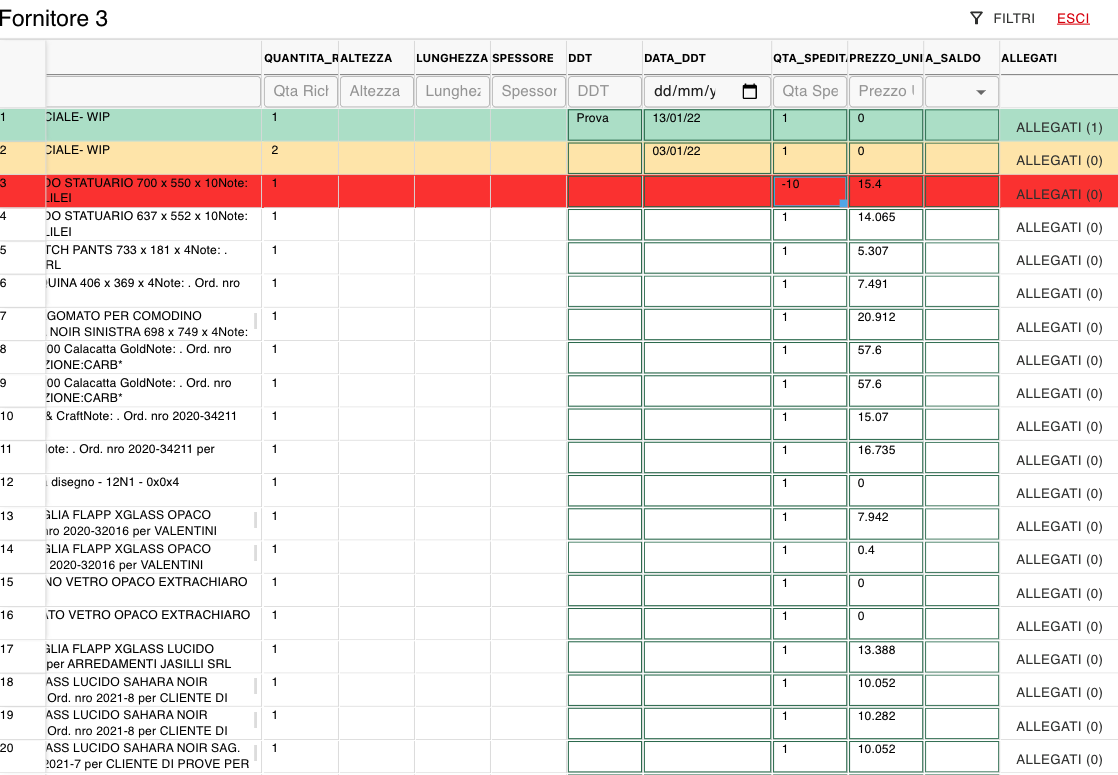
\includegraphics[scale=0.23]{screenshots/edi-user-dashboard.png}
    \caption{\emph{Dashboard} per l'utente di tipo fornitore}
    \label{fig:dashboard}
  \end{center}
\end{figure}

\newpage
\begin{figure}[!ht]
  \begin{center}
    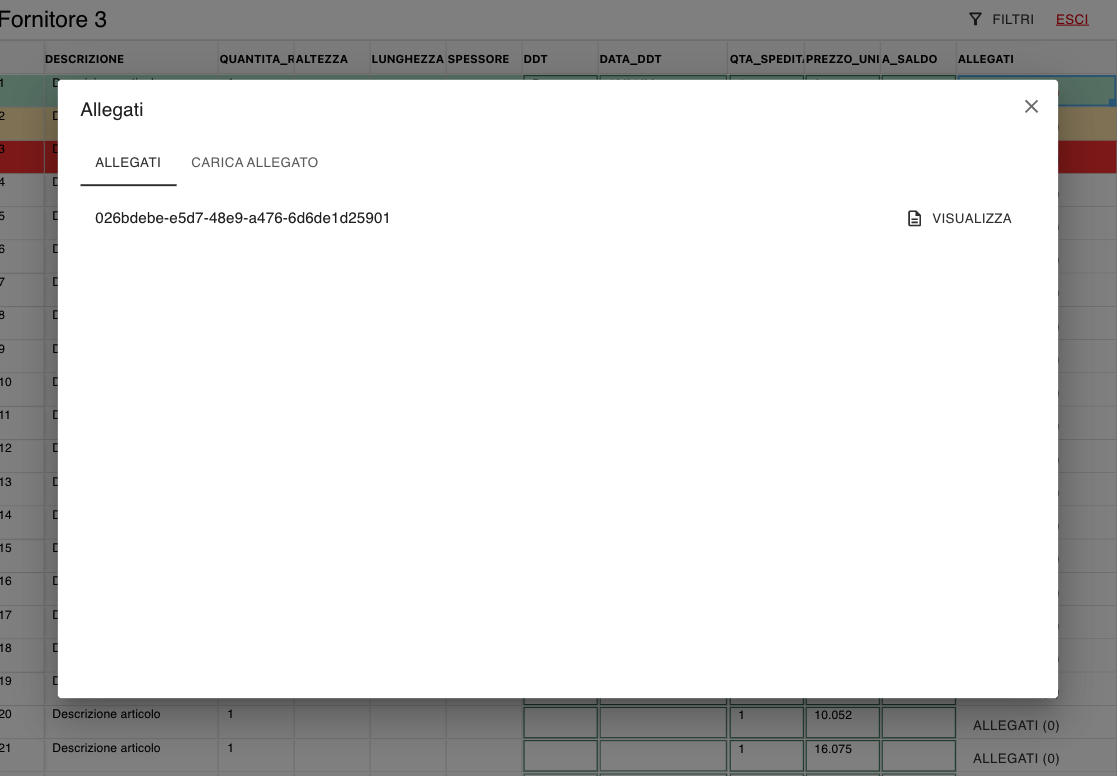
\includegraphics[scale=0.23]{screenshots/attachments-list.png}
    \caption{Lista degli allegati per un ordine}
    \label{fig:attachments-list}
  \end{center}
\end{figure}

\subsection{Personale}
Un utente facente parte del personale aziendale, la prima pagina che visualizza, come per gli utenti di tipo fornitore, è la \emph{dashboard}.
A differenza loro, però, come si osserva dalla figura \ref{fig:lago-dashboard}, mostra la lista di tutti i fornitori.
Per ogni fornitore nella lista è possibile visionare la relativa griglia degli ordini.
È possibile, inoltre, ricercare i fornitori mediante l'apposito campo di \emph{input}, situato sopra la lista.

\begin{figure}[!ht]
  \begin{center}
    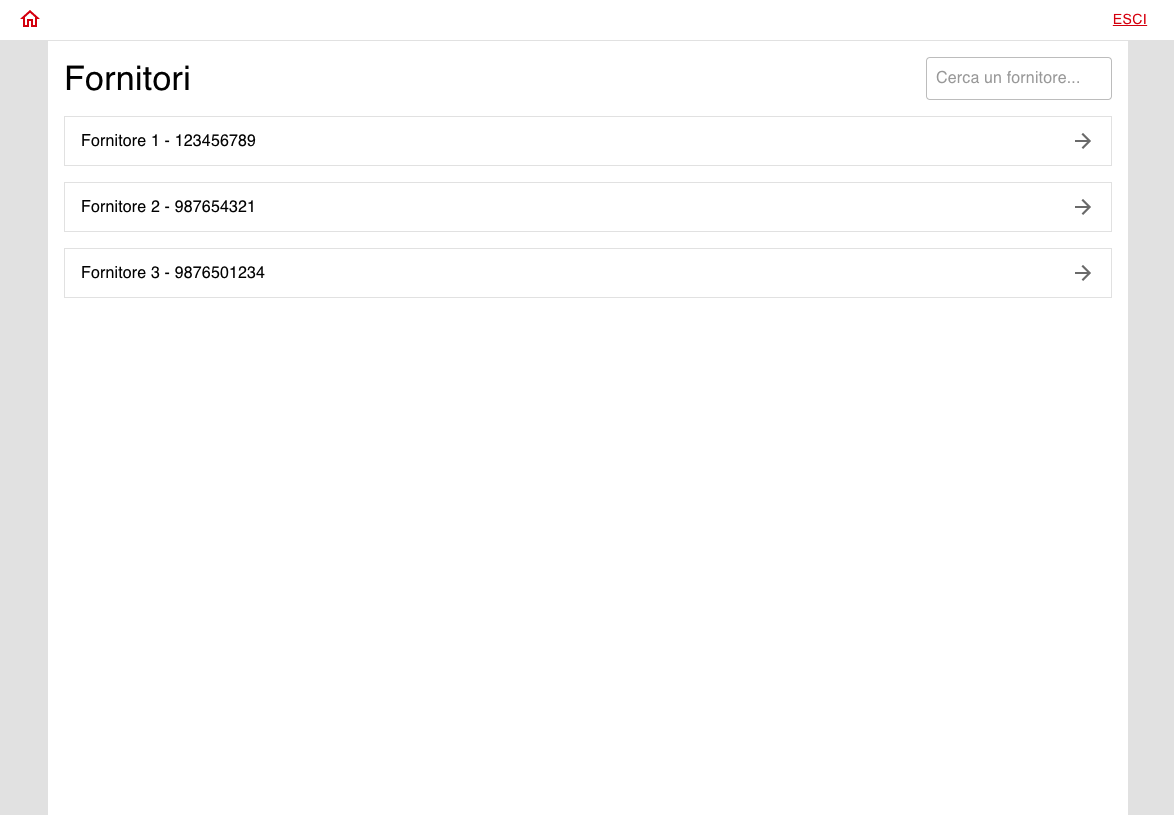
\includegraphics[scale=0.23]{screenshots/suppliers-list.png}
    \caption{\emph{Dashboard} per gli utenti di tipo personale}
    \label{fig:lago-dashboard}
  \end{center}
\end{figure}
\newpage
Un'altra funzionalità di cui godono gli utenti di tipo personale, è la possibilità di passare alla visualizzazione degli ordini di un altro fornitore direttamente dalla griglia.
La figura \ref{fig:supplier-swicher} mostra il componente che rende possibile questa operazione.

\begin{figure}[!ht]
  \begin{center}
    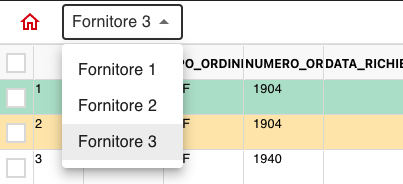
\includegraphics[scale=0.45]{screenshots/supplier-swicher.png}
    \caption{Componente per il cambio di fornitore dalla griglia}
    \label{fig:supplier-swicher}
  \end{center}
\end{figure}

La funzionalità, che risulta essere più importante però, è la possibilità di eliminare uno, o più, ordini dalla griglia.
Per potere fare ciò, è necessario prima selezionare tutti gli ordini che si intende eliminare, successivamente, si preme l'apposito pulsante, situato nella parte alta dell'applicazione, il quale apre una finestra di dialogo che richiede una conferma da parte dell'utente.
Una volta confermato, gli ordini selezionati verranno eliminati, mentre, in caso di annullamento, non sarà apportata alcuna modifica.
La figura \ref{fig:lago-grid-delete}, mostra gli ordini selezionati, pronti per poter essere eliminati.

\begin{figure}[!ht]
  \begin{center}
    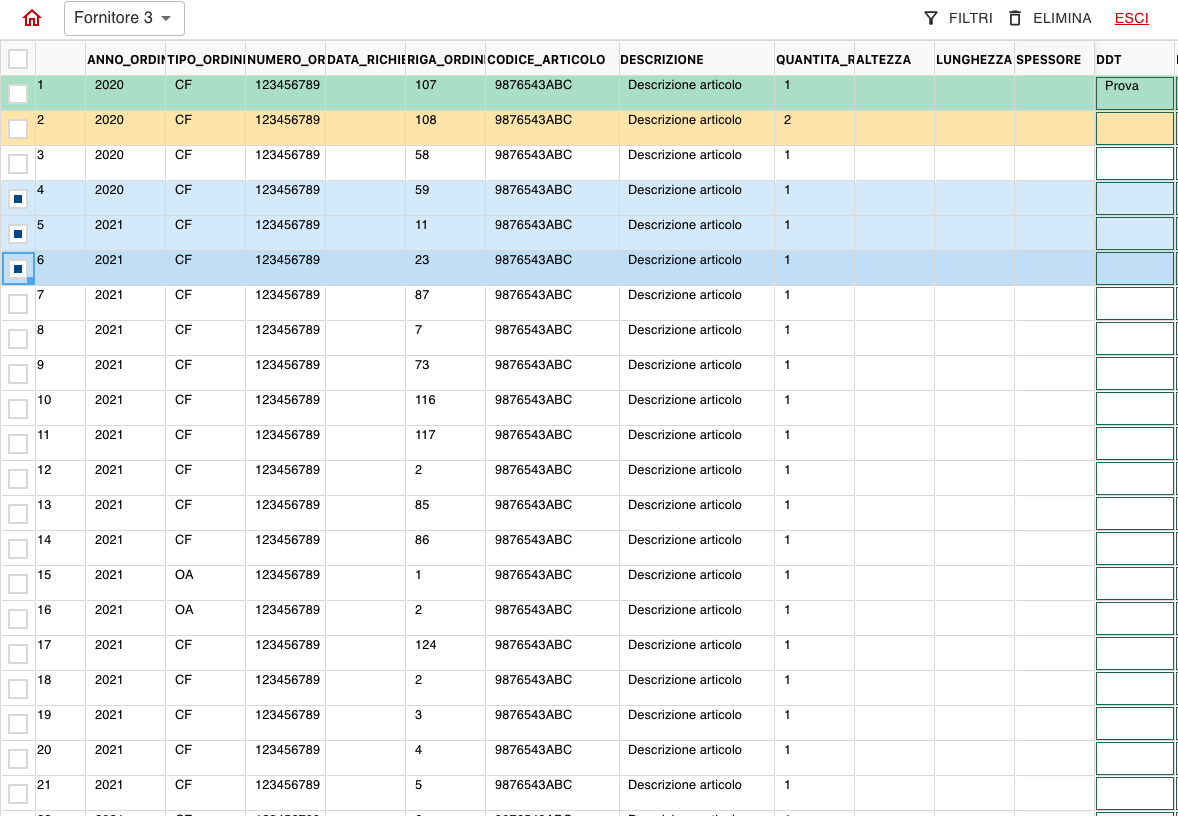
\includegraphics[scale=0.23]{screenshots/lago-grid-delete.png}
    \caption{Griglia con gli ordini da eliminare}
    \label{fig:lago-grid-delete}
  \end{center}
\end{figure}

\newpage
\subsection{Amministratori}
Gli utenti amministratori si differenziano degli altri in quanto hanno la possibilità di gestire gli utenti.
La \emph{dashboard} relativa a questo tipo di utenza, ha una struttura molto minimale, è costituita da due \emph{tabs} per accedere o alla lista degli utenti o alla lista dei fornitori.
La funzionalità più importante, è la possibilità di abilitare un utente. 
Ciò è possibile mediante l'apposito \emph{form}, presente all'interno della figura \ref{fig:users-list}, che diventa modificabile dopo che viene premuto il pulsante "Modifica".
Questo \emph{form} consente, inoltre, la possibilità di cambiare il ruolo dell'utente e, se l'utente è di tipo personale, renderlo un \emph{admin}, oppure, se è di tipo fornitore, assegnargli la visualizzazione dei propri ordini.

\begin{figure}[!ht]
  \begin{center}
    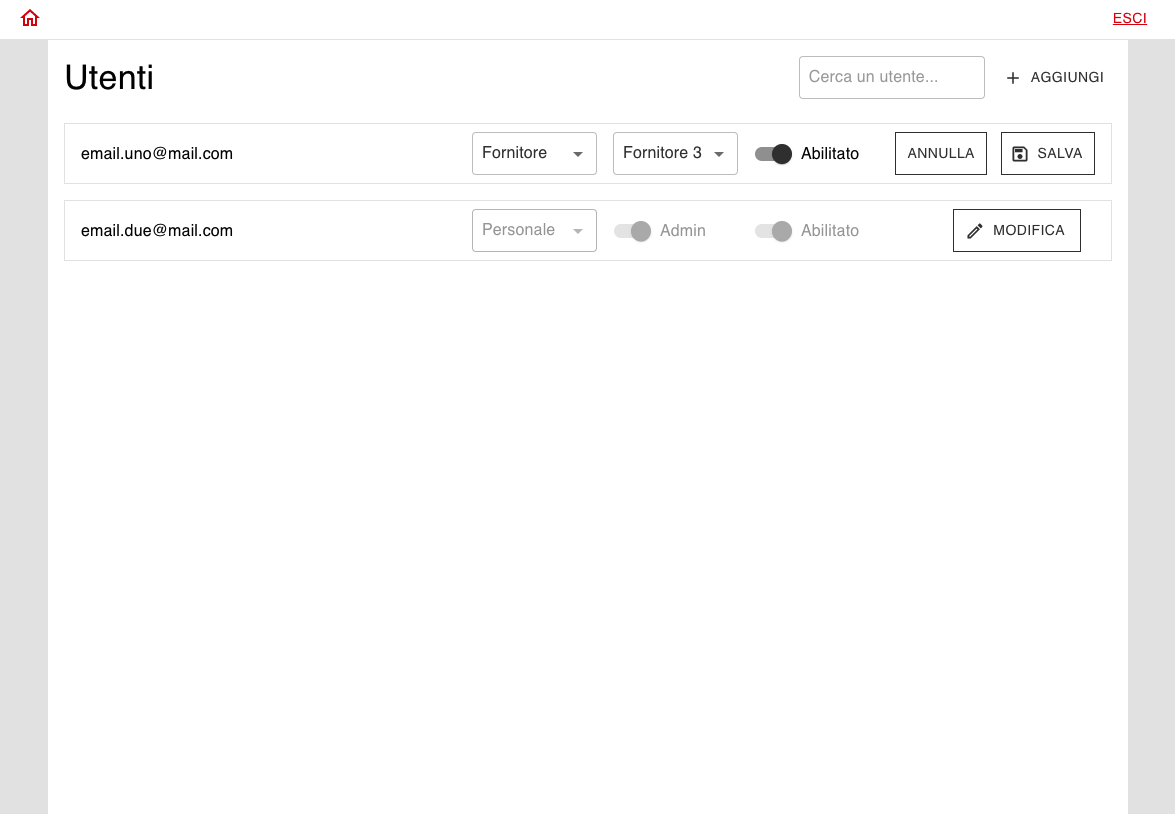
\includegraphics[scale=0.23]{screenshots/users-list.png}
    \caption{Lista degli utenti}
    \label{fig:users-list}
  \end{center}
\end{figure}

Un'altra funzionalità possibile per gli amministratori, è l'inserimento di uno, o più, nuovi utenti.
Ciò è possibile mediante l'apposito \emph{form}, visibile dopo aver premuto sul pulsante "Aggiungi".